\def\difficulty{3}
\sujet{Active contours}
\index{Segmentation!Active Contours}
\begin{note}This tutorials aims at introducing the active contours (a.k.a. snakes) method as originally presented in \cite{Kass1988}. It is a segmentation method based on the optimization of a contour that will converge to a specific object.\end{note}

\vspace*{-8pt}

\section{Definition}

\vspace*{-8pt}

\textls[-20]{A snake is a parametric curve $v(s)$ with $s\!\in\![0;1[$. The energy functional is represented by:}
$$E_{snake}=\int_0^1 E_{\textrm{int}}(v(s))\textrm{d}s+\int_0^1 E_{\textrm{ext}}(v(s)) \textrm{d}s.$$

The internal energy is detailed in Eq.\ref{eq:active_contours:enonce:energy}. The first order derivation constrains the length of the curve, 
the second order derivation constrains the curvature. The parameters $\alpha$ and $\beta$ a priori depend on $s$, but for simplicity, constant values will be taken.
\begin{equation}E_{\textrm{int}}(v(s)) = \frac{1}{2}\bigg(\underbrace{\alpha(s)|v'(s)|^2}_{length} + \underbrace{\beta(s)|v''(s)|^2}_{curvature}\bigg)
 \label{eq:active_contours:enonce:energy}
\end{equation}

The snake will be attracted by some edges points from the external energy (the image to be segmented). The, the energy functional will be in a local minimum: 
it is shown that the Euler-Lagrange equation is satisfied:
$$-\alpha v^{(2)} + \beta v^{(4)}+\nabla E_\textrm{ext}=0$$
with $v^{(2)}$ and $v^{(4)}$ denoting the 2nd and 4th order derivatives. To solve this equation, the gradient descent method is employed: the snake is 
now transformed into a function of the position $s$ and the time $t$, with $F_\textrm{ext}=-\nabla E_\textrm{ext}$
$$\frac{\partial s}{\partial t} = \alpha v^{(2)} - \beta v^{(4)}+ F_\textrm{ext}$$

\begin{figure}[H]
 \centering\caption{Illustration of the active contours segmentation method. Two energies are at stake: internal energies depend only on the snake shape and control points, external energies are related to the image properties.}%
 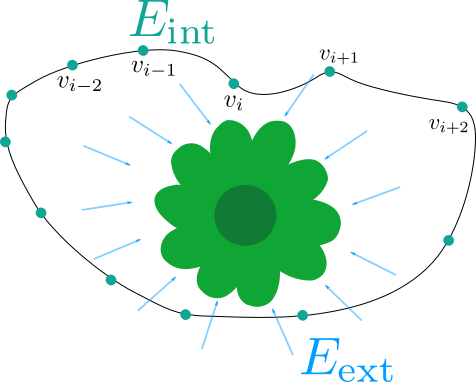
\includegraphics[width=6cm]{snake.pdf}
 \label{fig:active_contours:enonce:snake}
\end{figure}

\section{Numerical resolution}
The spatial derivatives are approximated with the finite difference method, and the snake is now composed of $n$ points, $i\in[1;n]$:

\begin{eqnarray*}
x^{(2)}&=&x_{i-1}-2x_i+x_{i+1} \\
x^{(4)}&=&x_{i-2}-4x_{i-1}+6x_i-4x_{i+1}+x_{i+2}
\end{eqnarray*}

The gradient descent method can be written as, with $\gamma$ being the time step and controls the convergence speed:
\begin{eqnarray*}
\frac{x_t-x_{t-1}}{\gamma} &=& A\cdot x_t + f_x(x_{t-1}, y_{t-1})\\
\frac{y_t-y_{t-1}}{\gamma} &=& A\cdot y_t + f_y(x_{t-1}, y_{t-1}) 
\end{eqnarray*}
with

$$A=\left[\begin{smallmatrix}
 -2\alpha-6\beta & \alpha+4\beta  & -\beta        &        0 &\cdots          & 0        & -\beta & \alpha+4\beta \\
 \alpha+4\beta   &-2\alpha-6\beta & \alpha+4\beta & -\beta   & 0   &\cdots          &     0   & -\beta        \\
 -\beta          & \alpha+4\beta  &-2\alpha-6\beta& \alpha+4\beta  & -\beta        & 0        &\cdots   & 0               \\
 0               &-\beta          & \alpha+4\beta &-2\alpha-6\beta & \alpha+4\beta & -\beta   & 0      & \cdots \\
 \vdots          &                &     \ddots    &    \ddots      &   \ddots      &  \ddots  &        &   \vdots \\
 0 &     \cdots         &-\beta          & \alpha+4\beta &-2\alpha-6\beta & \alpha+4\beta & -\beta   & 0 \\
0 & \cdots         &0              &-\beta          & \alpha+4\beta &-2\alpha-6\beta & \alpha+4\beta & -\beta \\
-\beta & 0 & \cdots &0             &-\beta          & \alpha+4\beta &-2\alpha-6\beta & \alpha+4\beta \\
\alpha+4\beta & -\beta & 0 & \cdots       &0       &-\beta          & \alpha+4\beta &-2\alpha-6\beta  \\
\end{smallmatrix}\right]$$

The forces $f_x$ and $f_y$ are the components of $F_{\textrm{ext}}$. 
For example for an image $I$, if $*$ denotes the convolution and 
$G_\sigma$ a gaussian kernel of standard deviation $\sigma$:
$$F_{\textrm{ext}}=-\nabla (\|\nabla(G_\sigma * I)\|)$$

\begin{qbox}
\begin{itemize}\item Generate a binary image (of size $n\times n$ pixels, with values 0 and 1) containing a disk (of a radius $R$).
 \item Generate the initial contour as an ellipse, with the same center as the disk.
 \item Generate the pentadiagonal matrix $A$. The different parameters can be $\alpha=10^{-5}$ and $\beta=0.05$.
 \item Program the iterations and visualize the results. For example, $\gamma=200$ and 1000 iterations may give an idea of the parameters to use.
\end{itemize}
\end{qbox}

